% Copyright 2006 by Till Tantau
%
% This file may be distributed and/or modified
%
% 1. under the LaTeX Project Public License and/or
% 2. under the GNU Free Documentation License.
%
% See the file doc/generic/pgf/licenses/LICENSE for more details.


\section{Declaring and Using Shadings}

\label{section-shadings}

\subsection{Overview}

A shading is an area in which the color changes smoothly between different
colors. Similarly to an image, a shading must first be declared before
it can be used. Also similarly to an image, a shading is put into a
\TeX-box. Hence, in order to include a shading in a |{pgfpicture}|,
you have to use |\pgftext| around it.

There are different kinds of shadings: horizontal, vertical, radial,
and functional shadings. However, you can rotate and clip shadings
like any other graphics object, which allows you to create more
complicated shadings. Horizontal shadings could be created by rotating
a vertical shading by 90 degrees, but explicit commands for creating both
horizontal and vertical shadings are included for convenience.

Once you have declared a shading, you can insert it into text using
the command |\pgfuseshading|. This command cannot be used directly in
a |{pgfpicture}|, you have to put a |\pgftext| around it. The second
command for using shadings, |\pgfshadepath|, on the other hand, can
only be used  inside |{pgfpicture}| environments. It will ``fill'' the
current path with the shading.

A horizontal shading is a horizontal bar of a certain height whose
color changes smoothly. You must at least specify the colors at the
left and at the right end of the bar, but you can also add color
specifications for points in between. For example, suppose you
which to create a bar that is red at the left end, green in the
middle, and blue at the end. Suppose you would like the bar to be 4cm
long. This could be specified as follows:
\begin{codeexample}[code only]
rgb(0cm)=(1,0,0); rgb(2cm)=(0,1,0); rgb(4cm)=(0,0,1)
\end{codeexample}
This line means that at 0cm (the left end) of the bar, the color
should be red, which has red-green-blue (rgb) components (1,0,0). At
2cm, the bar should be green, and at 4cm it should be blue.
Instead of |rgb|, you can currently also specify |gray| as
color model, in which case only one value is needed, or |color|,
in which case you must provide the name of a color in parentheses. In
a color specification the individual specifications must 
be separated using a semicolon, which may be followed by a whitespace
(like a space or a newline). Individual specifications must be given
in increasing order. 


\subsection{Declaring Shadings}

\begin{command}{\pgfdeclarehorizontalshading\oarg{color list}\marg{shading
      name}\marg{shading height}\marg{color specification}}
  Declares a horizontal shading named \meta{shading name} of the specified
  \meta{height} with the specified colors. The length of the bar is
  deduced automatically from the maximum dimension in the specification.

\begin{codeexample}[]
\pgfdeclarehorizontalshading{myshadingA}
  {1cm}{rgb(0cm)=(1,0,0); color(2cm)=(green); color(4cm)=(blue)}
\pgfuseshading{myshadingA}
\end{codeexample}

  The effect of the \meta{color list}, which is a
  comma-separated list of colors, is the following: Normally, when
  this list is empty, once a shading has been declared, it becomes
  ``frozen.'' This means that even if you change a color that was used
  in the declaration of the shading later on, the shading will not
  change. By specifying a \meta{color list} you can specify
  that the shading should be recalculated whenever one of the colors
  listed in the list changes (this includes effects like color
  mixins). Thus, when you specify a \meta{color list},
  whenever the shading is used, \pgfname\ first converts the colors in the
  list to \textsc{rgb} triples using the current values of the
  colors and taking any mixins and blends into account. If the
  resulting \textsc{rgb} triples have not yet been   used, a new
  shading is internally created and used. Note that if the 
  option \meta{color list} is used, then no shading is created until
  the first use of |\pgfuseshading|. In particular, the colors
  mentioned in the shading need not be defined when the declaration is
  given.

  When a shading is recalculated because of a change in the
  colors mentioned in \meta{color list}, the complete shading
  is recalculated. Thus even colors not mentioned in the list will be
  used with their current values, not with the values they had upon
  declaration.
  
\begin{codeexample}[]
\pgfdeclarehorizontalshading[mycolor]{myshadingB}
  {1cm}{rgb(0cm)=(1,0,0); color(2cm)=(mycolor)}
\colorlet{mycolor}{green}
\pgfuseshading{myshadingB}
\colorlet{mycolor}{blue}
\pgfuseshading{myshadingB}
\end{codeexample}
\end{command}


\begin{command}{\pgfdeclareverticalshading\oarg{color list}\marg{shading
      name}\marg{shading width}\marg{color specification}}
   Declares a vertical shading named \meta{shading name} of the
   specified \meta{width}. The height of the bar is deduced
   automatically. The effect of \meta{color list} is the same as for
   horizontal shadings.

\begin{codeexample}[]
\pgfdeclareverticalshading{myshadingC}
  {4cm}{rgb(0cm)=(1,0,0); rgb(1.5cm)=(0,1,0); rgb(2cm)=(0,0,1)}
\pgfuseshading{myshadingC}
\end{codeexample}
\end{command}


\begin{command}{\pgfdeclareradialshading\oarg{color list}\marg{shading
      name}\marg{center point}\marg{color specification}}
  Declares an radial shading. A radial shading is a circle whose inner
  color changes as specified by the color specification. Assuming that
  the center of the shading is at the origin, the color of the center
  will be the color specified for 0cm and the color of the border of
  the circle will be the color for the maximum dimension given in
  the \meta{color specified}. This maximum will also be the radius of
  the circle. If the \meta{center point} is not at the 
  origin, the whole shading inside the circle (whose size remains
  exactly the same) will be distorted such that the given center now
  has the color specified for 0cm. The effect of \meta{color list} is
  the same as for horizontal shadings. 

\begin{codeexample}[]  
\pgfdeclareradialshading{sphere}{\pgfpoint{0.5cm}{0.5cm}}%
  {rgb(0cm)=(0.9,0,0);
   rgb(0.7cm)=(0.7,0,0);
   rgb(1cm)=(0.5,0,0);
   rgb(1.05cm)=(1,1,1)}
\pgfuseshading{sphere}
\end{codeexample}
\end{command}


\begin{command}{\pgfdeclarefunctionalshading\oarg{color list}\marg{shading
      name}\marg{lower left corner}\marg{upper right corner}\marg{init code}\marg{type 4 function}}
  \emph{Warning: These shadings are the least portable of all and they
  put the heaviest burden of the renderer. They are slow and,
  possibly, will not print correctly!}

  This command creates a \emph{functional shading}. For such a
  shading, the color of each point is calculated by calling a function
  that gets the coordinates of the point as input and yields the
  color as an output. Note that the function is evaluated by the 
  \emph{renderer}, not by \pgfname\ or \TeX or someone else at
  compile-time. This means that the evaluation of this function has to
  be done \emph{extremely quickly} and the funciton should be
  \emph{very simple}. For this reason, only a very restricted set of
  operations are possible in the function and functions should be
  kept small. Any errors in the function will only be noticed by the
  renderer.

  The syntax for specifying functions is the following: You use a
  simplified form of a subset of the PostScript language. This subset
  will be understood by the PDF-renderer (yes, PDF-renderers do
  have a basic understanding of PostScript) and also by PostScript
  renders. This subset is detailed in Seciton 3.9.4 of the
  PDF-specification (version 1.7). In essence, the specificaiton
  states that these functions may contain ``expressions involving
  integers, real numbers, and boolean values only. There are no
  composite data structures such as strings or arrays, no procedures,
  and no variables or names.'' The allowed operators are (exactly) the
  following: \texttt{abs}, \texttt{add}, \texttt{atan},
  \texttt{ceiling}, \texttt{cos}, \texttt{cvi}, \texttt{cvr},
  \texttt{div}, \texttt{exp}, \texttt{floor}, \texttt{idiv},
  \texttt{ln}, \texttt{log}, \texttt{mod}, \texttt{mul}, \texttt{neg},
  \texttt{round}, \texttt{sin}, \texttt{sqrt}, \texttt{sub},
  \texttt{truncate}, \texttt{and}, \texttt{bitshift}, \texttt{eq},
  \texttt{false}, \texttt{ge}, \texttt{gt}, \texttt{le}, \texttt{lt},
  \texttt{ne}, \texttt{not}, \texttt{or}, \texttt{true}, \texttt{xor},
  \texttt{if}, \texttt{ifelse}, \texttt{copy}, \texttt{dup},
  \texttt{exch}, \texttt{index}, \texttt{pop}.

  When the function is evaluated, the top two stack elements are the
  coordinates of the point for which the color should be computed. The
  coordinates are dimensionless and given in big points, so for the
  coordinate $(50bp, 72.27pt)$ the top two stack elements would be
  \texttt{50.0} and \texttt{72.0}. Ohterwise, the (virtual) stack is
  empty (or should be treated as if it were empty). The function
  should then replace these two values by three values, representing
  the red, green, and blue color of the point. The numbers should be
  real values, not integers since Apple's PDF renderer is broken in
  this regard (use cvr at the end if necessary).

  Conceptually, the function will be evaluated once for each point of
  the rectangle \meta{lower left corner} to \meta{upper right corner},
  which should be a \pgfname-point expression like
  |\pgfpoint{100bp}{100bp}|. A renderer may choose to evaluate the
  function at less points, but, in principle, the function will be
  evaluated for each pixel independently. 

  Because of the rather difficult PostScript syntax, use this macro
  only \emph{if you know what you are doing} (or if you are
  advanterous, of course). 

  As for other shadings, the optional \meta{color list} is used to
  determine whether a shading needs to be recalculated when a color
  has changed.

  The \meta{init code} is executed each time a shading is
  (re)calculated. Typically, it will contain code to extract
  coordinates from colors (see below).

  Inside the PostScript function \meta{type 4 function} you cannot use
  colors directly. Rather, you must push the color components on the
  stack. For this, it is useful to call |\pgfshadecolorrgb| in the
  \meta{init code}. The macro takes a color name as input and stores
  the color's red/green/blue components real numbers between 0.0 and
  1.0 separated by spaces (which is exactly what you need if you want
  to push it on a stack) in a macro. You can then use this macro in
  the argument \meta{type 4 function}.

\begin{codeexample}[]
\pgfdeclarefunctionalshading{twospots}
    {\pgfpointorigin}{\pgfpoint{4cm}{4cm}}{}{
  % Save coordinates for later
  2 copy
  % Compute distance from (40bp,45bp), with x doubled
  45 sub dup mul exch
  40 sub dup mul 0.5 mul add sqrt
  % expontial decay
  dup mul neg 1.0005 exch exp 1.0 exch sub
  % Compute distance form (70bp,70bp) from stored coordiante, scaled
  3 1 roll
  70 sub dup mul .5 mul exch
  70 sub dup mul add sqrt
  % Decay
  dup mul neg 1.002 exch exp 1.0 exch sub
  % red component
  1.0 3 1 roll
}
\pgfuseshading{twospots}
\end{codeexample}

\begin{codeexample}[]
\pgfdeclarefunctionalshading[mycol]{sweep}{\pgfpoint{-1cm}{-1cm}}
{\pgfpoint{1cm}{1cm}}{\pgfshadecolortorgb{mycol}{\myrgb}}{
  2 copy        % whirl
  atan
  3 1 roll
  dup mul exch
  dup mul add sqrt
  30 mul
  1 index add
  sin
  1 add 2 div  
  dup
  \myrgb        % push mycol
  5 4 roll      % multiply all components by calculated value
  mul
  3 1 roll
  3 index
  mul
  3 1 roll
  4 3 roll
  mul
  3 1 roll
}
\colorlet{mycol}{white}%
\pgfuseshading{sweep}%
\colorlet{mycol}{red}%
\pgfuseshading{sweep}
\end{codeexample}
\end{command}


\subsection{Using Shadings}
\label{section-shading-a-path}

\begin{command}{\pgfuseshading\marg{shading name}}
  Inserts a previously declared shading into the text. If you wish to
  use it in a |pgfpicture| environment, you should put a |\pgfbox|
  around it.
  
\begin{codeexample}[]
\begin{pgfpicture}
  \pgfdeclareverticalshading{myshadingD}
    {20pt}{color(0pt)=(red); color(20pt)=(blue)}
  \pgftext[at=\pgfpoint{1cm}{0cm}]  {\pgfuseshading{myshadingD}}
  \pgftext[at=\pgfpoint{2cm}{0.5cm}]{\pgfuseshading{myshadingD}}
\end{pgfpicture}
\end{codeexample}
\end{command}

\begin{command}{\pgfshadepath\marg{shading name}\marg{angle}}
  This command must be used inside a |{pgfpicture}| environment. The
  effect is a bit complex, so let us go over it step by step.

  First, \pgfname\ will setup a local scope.

  Second, it uses the current path to clip everything inside this
  scope. However, the current path is once more available after the
  scope, so it can be used, for example, to stroke it.

  Now, the \meta{shading name} should be a shading whose width and
  height are 100\,bp, that is, 100 big points. \pgfname\ has a look at
  the bounding box of the current path. This bounding box is computed
  automatically when a path is computed; however, it can sometimes be
  (quite a bit) too large, especially when complicated curves are
  involved. 

  Inside the scope, the low-level transformation matrix is modified.
  The center of the shading is translated (moved) such that it lies on
  the center of the bounding box of the path. The low-level coordinate
  system is also scaled such that the shading ``covers'' the shading (the 
  details are a bit more complex, see below). Then, the coordinate
  system is rotated by \meta{angle}. Finally, if the macro 
  |\pgfsetadditionalshadetransform| has been used, an additional
  transformation is applied. 

  After everything has been set up, the shading is inserted. Due to
  the transformations and clippings, the effect will be that  the
  shading seems to ``fill'' the path.

  If both the path and the shadings were always rectangles and if
  rotation were never involved, it would be easy to scale shadings
  such they always cover the path. However, when a vertical shading is
  rotated, it must obviously be ``magnified'' so that it
  still covers the path. Things get worse when the path is not a
  rectangle itself.

  For these reasons, things work slightly differently ``in reality.''
  The shading is scaled and translated such that the
  the point $(50\mathrm{bp},50\mathrm{bp})$, which is the middle of
  the shading, is at the middle of the path and such that the the
  point $(25\mathrm{bp},25\mathrm{bp})$ is at the lower left corner of
  the path and that  $(75\mathrm{bp},75\mathrm{bp})$  is at upper
  right corner.

  In other words, only the center quarter of the shading will actually
  ``survive the clipping'' if the path is a rectangle. If the path is
  not a rectangle, but, say, a circle, even less is seen of the
  shading. Here is an example that demonstrates this effect:

\begin{codeexample}[]
\pgfdeclareverticalshading{myshadingE}{100bp}    
 {color(0bp)=(red); color(25bp)=(green);  color(75bp)=(blue);  color(100bp)=(black)}
\pgfuseshading{myshadingE} 
\hskip 1cm
\begin{pgfpicture}
  \pgfpathrectangle{\pgfpointorigin}{\pgfpoint{2cm}{1cm}}
  \pgfshadepath{myshadingE}{0}
  \pgfusepath{stroke}
  \pgfpathrectangle{\pgfpoint{3cm}{0cm}}{\pgfpoint{1cm}{2cm}}
  \pgfshadepath{myshadingE}{0}
  \pgfusepath{stroke}
  \pgfpathrectangle{\pgfpoint{5cm}{0cm}}{\pgfpoint{2cm}{2cm}}
  \pgfshadepath{myshadingE}{45}
  \pgfusepath{stroke}
  \pgfpathcircle{\pgfpoint{9cm}{1cm}}{1cm}
  \pgfshadepath{myshadingE}{45}
  \pgfusepath{stroke}
\end{pgfpicture}
\end{codeexample}

  As can be seen above in the last case, the ``hidden'' part of the
  shading actually \emph{can} become visible if the shading is
  rotated. The reason is that it is scaled as if no rotation took
  place, then the rotation is done.

  The following graphics show which part of the shading are actually
  shown: 

\begin{codeexample}[]
\pgfdeclareverticalshading{myshadingF}{100bp}    
 {color(0bp)=(red); color(25bp)=(green);  color(75bp)=(blue);  color(100bp)=(black)}
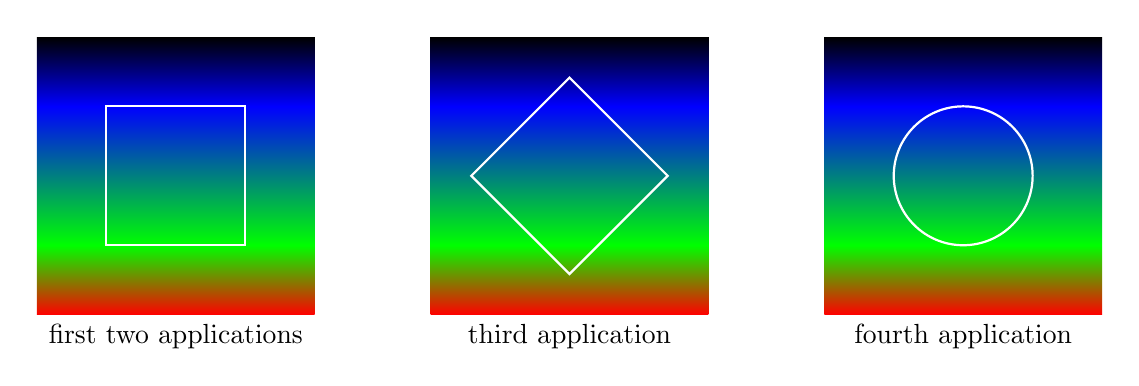
\begin{tikzpicture}
  \draw (50bp,50bp) node {\pgfuseshading{myshadingF}};
  \draw[white,thick] (25bp,25bp) rectangle (75bp,75bp);
  \draw (50bp,0bp) node[below] {first two applications};

  \begin{scope}[xshift=5cm]
    \draw (50bp,50bp) node{\pgfuseshading{myshadingF}};
    \draw[rotate around={45:(50bp,50bp)},white,thick] (25bp,25bp) rectangle (75bp,75bp);
    \draw (50bp,0bp) node[below] {third application};
  \end{scope}

  \begin{scope}[xshift=10cm]
    \draw (50bp,50bp) node{\pgfuseshading{myshadingF}};
    \draw[white,thick] (50bp,50bp) circle (25bp);
    \draw (50bp,0bp) node[below] {fourth application};
  \end{scope}
\end{tikzpicture}
\end{codeexample}
  
  An advantage of this approach is that when you rotate a radial
  shading, no distortion is introduced:

\begin{codeexample}[]
\pgfdeclareradialshading{ballshading}{\pgfpoint{-10bp}{10bp}}
 {color(0bp)=(red!15!white); color(9bp)=(red!75!white);
 color(18bp)=(red!70!black); color(25bp)=(red!50!black); color(50bp)=(black)}
\pgfuseshading{ballshading}
\hskip 1cm
\begin{pgfpicture}
  \pgfpathrectangle{\pgfpointorigin}{\pgfpoint{1cm}{1cm}}
  \pgfshadepath{ballshading}{0}
  \pgfusepath{}
  \pgfpathcircle{\pgfpoint{3cm}{0cm}}{1cm}
  \pgfshadepath{ballshading}{0}
  \pgfusepath{}
  \pgfpathcircle{\pgfpoint{6cm}{0cm}}{1cm}
  \pgfshadepath{ballshading}{45}
  \pgfusepath{}
\end{pgfpicture}
\end{codeexample}

  If you specify a rotation of $90^\circ$
  and if the path is not a square, but an elongated rectangle,  the
  ``desired'' effect results: The shading will exactly vary between
  the colors at the 25bp and 75bp boundaries. Here is an example:
  
\begin{codeexample}[]
\pgfdeclareverticalshading{myshadingG}{100bp}    
 {color(0bp)=(red); color(25bp)=(green);  color(75bp)=(blue);  color(100bp)=(black)}
\begin{pgfpicture}
  \pgfpathrectangle{\pgfpointorigin}{\pgfpoint{2cm}{1cm}}
  \pgfshadepath{myshadingG}{0}
  \pgfusepath{stroke}
  \pgfpathrectangle{\pgfpoint{3cm}{0cm}}{\pgfpoint{2cm}{1cm}}
  \pgfshadepath{myshadingG}{90}
  \pgfusepath{stroke}
  \pgfpathrectangle{\pgfpoint{6cm}{0cm}}{\pgfpoint{2cm}{1cm}}
  \pgfshadepath{myshadingG}{45}
  \pgfusepath{stroke}
\end{pgfpicture}
\end{codeexample}


  As a final example, let us define a ``rainbow spectrum'' shading for
  use with \tikzname.
\begin{codeexample}[]
\pgfdeclareverticalshading{rainbow}{100bp}
 {color(0bp)=(red); color(25bp)=(red); color(35bp)=(yellow);
  color(45bp)=(green); color(55bp)=(cyan); color(65bp)=(blue);
  color(75bp)=(violet); color(100bp)=(violet)}
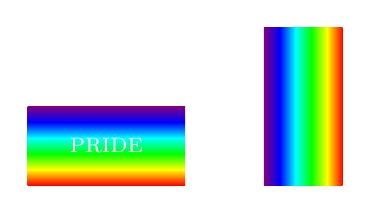
\begin{tikzpicture}[shading=rainbow]
  \shade (0,0) rectangle node[white] {\textsc{pride}} (2,1);
  \shade[shading angle=90] (3,0) rectangle +(1,2);
\end{tikzpicture}
\end{codeexample}

  Note that rainbow shadings are \emph{way} to colorful in almost all
  applications. 
\end{command}

\begin{command}{\pgfsetadditionalshadetransform\marg{transformation}}
    This command allows you to specify an additional transformation
    that should be applied to shadings when the |\pgfshadepath|
    command is used. The \meta{transformation} should be
    transformation code like |\pgftransformrotate{20}|.  
\end{command}

%%% Local Variables: 
%%% mode: latex
%%% TeX-master: "pgfmanual"
%%% End: 
